% LaTeX Datei für Projektberichte
\documentclass[12pt,a4paper,oneside]{article}

%---------------------------------------------------------------
%	Pakete
%---------------------------------------------------------------

\usepackage{tikz}
\usepackage[ngerman]{babel}            %   neue deutsche Rechtschreibung
\usepackage[utf8]{inputenc}
\usepackage[T1]{fontenc}
\usepackage{subfigure} 

\usepackage{color}
\usepackage{graphicx}
\usepackage{setspace}
\usepackage[title,titletoc,toc]{appendix}
\usepackage{geometry}
\geometry{a4paper,left=19mm,right=19mm, top=25mm, bottom=25mm}
\usetikzlibrary{shapes.geometric, arrows}


%---------------------------------------------------------------
% Dokumentenanfang:
%---------------------------------------------------------------
\begin{document}                            % Dokumentenanfang
	\usetikzlibrary{shapes,arrows}
\begin{spacing}{1.15}                       % Zeilenabstand 1,15

	\begin{titlepage}

\begin{flushleft}
	
\includegraphics[height=1.5cm]{figs/LKR_Logo.png}
	\hfill
	%\includegraphics[height=1.5cm]{figs/MZH_Logo.png}
	%\hfill
	
\includegraphics[height=1.5cm]{figs/LUH_Logo.jpg}
\end{flushleft}

\vspace{10mm} 
\begin{center}
\Large{Vorlesung/Experimentelle \"Ubung: 

Programmierung mechatronischer Systeme

\vspace{5mm}

\textbf{Hausarbeit}}

\vspace{5mm}
\textbf{\LARGE{Raspberry Pi Roboter ("French Bulldog")}}
\end{center}

\vfill
% hier könnt ihr ein Bild eurer Roboters einfügen
\begin{center}
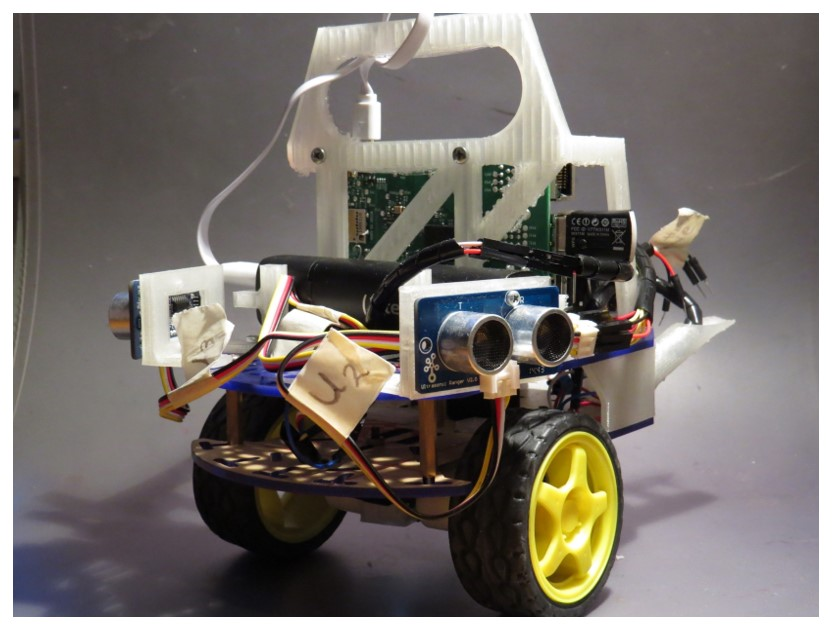
\includegraphics[width = 80mm]{figs/PiRobot.jpg}
\end{center}

\vfill

\begin{center}
\begin{tabular}{c c}
\large{Tobias Gieseking} & \large{Nils Melchert}\\
\large{Matrikelnummer 2883510} & \large{Matrikelnummer 2869520}
\end{tabular}
\end{center}
\vspace{15mm}

\begin{tabular}{l}
\large{Sommersemester 2016}\\
\large{Hannover, 15.07.2016}
\end{tabular}


\vspace{15mm}
{\large
\begin{tabular}{l l}
Dozentin:  & Prof. Dr.-Ing. Jessica Burgner\\
Betreuer: & M.Sc. Ernar Amanov und M.Sc. Carolin Fellmann\\
\end{tabular}
}

\end{titlepage}

    \clearpage
    \tableofcontents                        % Inhaltsverzeichnis 
    \thispagestyle{empty}
    \clearpage   
	\setcounter{page}{1}
	%-----------------------------
	% Einleitung
	%-----------------------------	
	\section{Einleitung}
	\textit{ca. 1 Seite}
	
	\textit{Einleitung zum Projekt. Motivation, Ziele die ihr mit eurem Roboter hattet, Herausforderungen...}
	
	In kursiv sind Vorgaben für eure Hausarbeit angegeben, bzw. Anregungen was in dem jeweiligem Abschnitt stehen sollte. Eure Hausarbeit sollte mindestens 13 Seiten haben, maximal 18 Seiten; der Anhang, sowie die Titelseite, Inhaltsverzeichnis und das Literaturverzeichnis werden \textbf{nicht} zur Seitenzahl gezählt. Unterstützt eure Hausarbeit visuell mit Fotos und Abbildungen, Tabellen etc. 
	
Generell gilt: Quellen bitte angeben! \cite{Dem13}
	
%-----------------------------
% Der Roboter
%-----------------------------
\section{Der Roboter}
\textit{3 bis 5 Seiten}	
	
\textit{In diesem Abschnitt soll euer Roboter hardwareseitig beschrieben werden: Hardwarekomponenten, Elektronik, Schaltpläne. Welche Sensoren wurden ausgewählt und warum? Welche Eigenschaften hat der fertige Roboter? Gewicht, Maximalgeschwindigkeit,...}

\subsection{Mobile Plattform}

\subsection{Sensorik}

	

%-----------------------------
% Softwaretechnische Umsetzung
%-----------------------------
\section{Umsetzung der Meilensteine}

	
\subsection{Linie folgen}
\textit{}	

Im Rahmen des ersten Meilensteins, gilt es einer weißen Linie auf schwarzem Untergrund zu folgen. Der Linienverlauf beinhaltet dabei sowohl Geradeausverläufe, als auch Links- und Rechtsabbiegungen in Form von S-Kurven und 90-Grad-Abbiegungen. Zwei der in Kapitel 2.2 beschriebenen digitalen Infrarot-Spursensoren werden zur Ermittlung der Position des Roboters entlang der besagten Linie montiert und angeschlossen. Die Schnittstelle zum Auslesen der digitalen Signale der Sensoren liefert eine Klasse \textit{Liniensensor}, welche eine Methode zur Erfassung digitaler Pegel bereitstellt. Sie liest einen Anschlusspin des RaspberryPi aus und detektiert, ob sich der Roboter über weißem oder schwarzem Untergrund befindet. Für jeden Sensor wird ein Objekt des Typs \textit{Liniensensor} in der Klasse \textit{Mobileplatform} erstellt.

Zur Linienfahrt ergeben sich drei Ansätze, die auf der Orientierung besagter Spursensoren basieren: Das Verfolgen einer Linienkante, Platzierung beider Sensoren auf der Linie und Positionierung rechts und links neben der Linie. Im Rahmen dieser Arbeit wurde der letzte Ansatz gewählt, da er sich bei der Implementierung als robuster erwiesen hat und sich zugleich ein ruhigeres Fahrverhalten einstellte.

Basierend auf der zuvor genannten Lösungsstrategie, ergibt sich die Implementierung des Algorithmus. Ein Programmablaufplan dessen ist in Abbildung ... zu sehen. Er hat die Aufgabe die Sensoren während der Fahrt stets links und rechts neben der weißen Linie zu halten. Der Aufruf des Algorithmus erfolgt in der Klasse \textit{Mobileplatform} über eine ungetaktete While-Schleife, sodass kontinuierlich der Status beider Sensoren abgefragt wird. Detektieren die Liniensensoren beide schwarzen Untergrund, befinden sich die Sensoren in ihrer Soll-Position und der Roboter fährt geradeaus. Ist gibt der linke Sensor einen \textit{Low-Pegel} zurück, befindet sich dieser über weißem Untergrund. Der Roboter ist zu weit nach rechts abgewichen. Es folgt eine Korrektor der Ausrichtung anhand einer Linksdrehung. Analog Erfolgt bei einem \textit{Low-Pegel} des rechten Sensors eine Rechtsdrehung.

\begin{figure}[!htb]
	\centering
	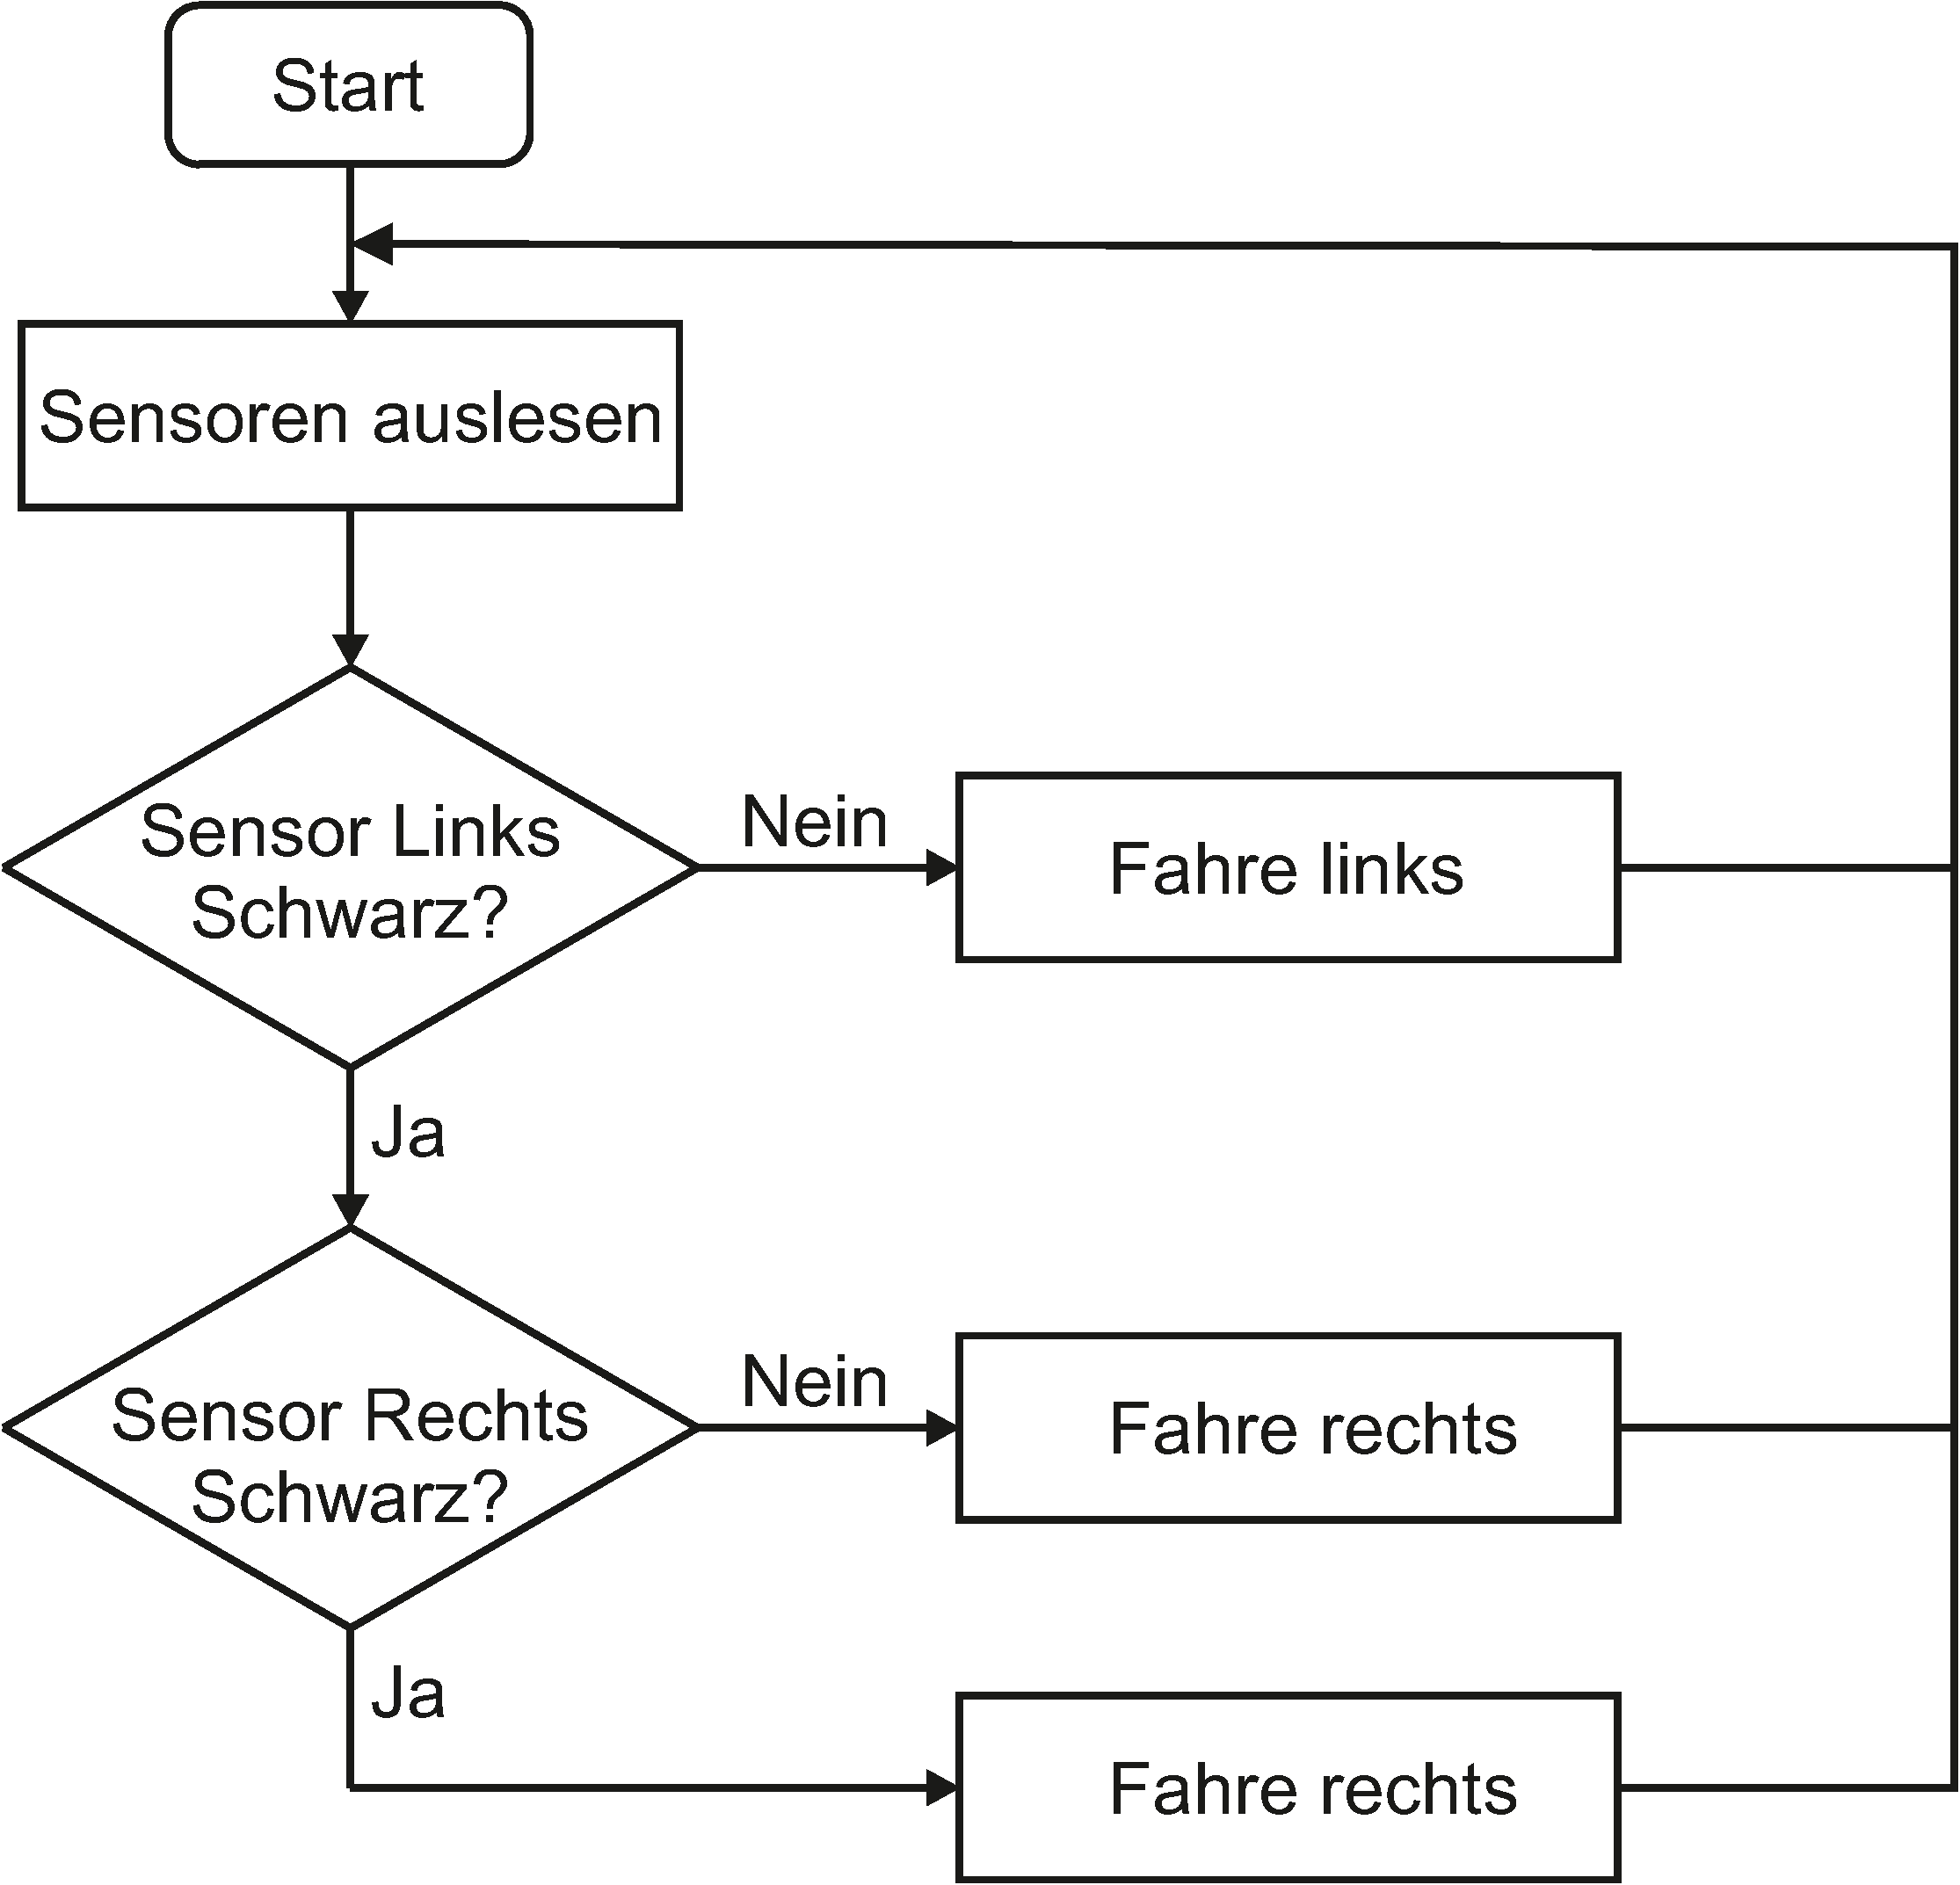
\includegraphics[scale=.3]{figs/PAP_Linie.pdf}
	\caption{Programmablaufplan der Linienfahrt}
	\label{fig:PAP_Linie}
\end{figure}


Die Bewältigung der Aufgabe lief mit dem gewählten Lösungsansatz problemlos. Dies ist unter anderem aber auch auf die stets nahezu konstante Breite der weißen Linie zurückzuführen. Sobald der Abstand der Sensoren geringer ist, als die besagte Breite, versagt die gewählte Lösungsstrategie. Unter dieser Bedingung ist erfahrungsgemäß der Ansatz zur Orientierung an Linienkanten zu wählen. \\
Zudem hatten hohe Geschwindigkeiten aufgrund der Massenträgheit zur Folge, dass der Roboter besonders bei 90-Grad-Abbiegungen nicht rechtzeitig abbremst und die Linie verlässt. Durch die Detektion schwarzen Untergrunds beider Sensoren, betrachtet der Algorithmus den Roboter in seiner Soll-Position und lässt ihn geradeaus fahren. Um diesem Versagen des Algorithmus entgegenzuwirken, wurde die Fahrtgeschwindigkeit angepasst.
%Abbildungen: PAP, Schematisch Lösungsstrategien, Linienverläufe

	
\subsection{Kreisfahrt}

Die Kreisfahrt war Bestandteil des zweiten Meilensteins. Unter Vorgabe eines Radius im Bereich von 15-35 Zentimeter, galt es den Roboter einen Kreis fahren zu lassen. Dieser durfte einen Toleranzbereich von $\pm$ 2cm nicht verlassen. Zur Überprüfung wurde ein Stift am Roboter befestigt, welcher auf einer Kreisschablone die gefahrene Strecke des Roboters aufzeichnet. Zwei der in Kapitel 2.2 beschriebenen Encoder wurden angeschlossen und eine Klasse \textit{Encoder} in \textit{Dcmotor} integriert(Siehe Abbildung ...). Des weiteren wurde eine Regelung der Geschwindigkeit in der Klasse \textit{Dcmotor} implementiert. Der Algorithmus zur Kreisfahrt wurde schließlich in eine Funktion geschrieben, die die Berechnung der Geschwindigkeiten beider Gleichstrommotoren realisiert. 

Über zwei Hall-Sensoren und ein Getriebe mit einer Übersetzung von 120:1 \cite{Dem13} ergeben sich pro Radumdrehung 1440 Signalflanken des Drehgebers. Über einen Zeitraum von $\Delta T = 0.1s$ werden Impulse $k$ gezählt und nach Gleichung \ref{eq:calcSpeed} unter Berücksichtigung des Raddurchmessers von $d = 0,063m$ zu einer Geschwindigkeit in SI-Basiseinheiten umgerechnet.

\begin{center}
\begin{equation}
v = \frac{k d \pi}{1440\Delta T}
\label{eq:calcSpeed}
\end{equation}
\end{center} 

Da der Signalpegel des Drehgebers im Zeitraum von 0,1 Sekunden ausreichend hoch ist, um eine Geschwindigkeit zu berechnen, kann Messrauschen durch ungenaue Fertigung der Encoder vernachlässigt werden. Demzufolge führt die Mittelwertbildung mehrerer Drehzahlsignale zu keiner Verbesserung in der Regelung.

Zur Regelung wird ein PID-Regler mit einer Taktrate von $10Hz$ implementiert. Somit wird bei jeder Erfassung der aktuellen Geschwindigkeit eine Änderung dieser durch den Regler vorgenommen. Abbildung \ref{fig:PID_controller}  zeigt ein Blockschaltbild des verwendeten PID-Reglers. 

\begin{figure}[!htb]
	\centering
	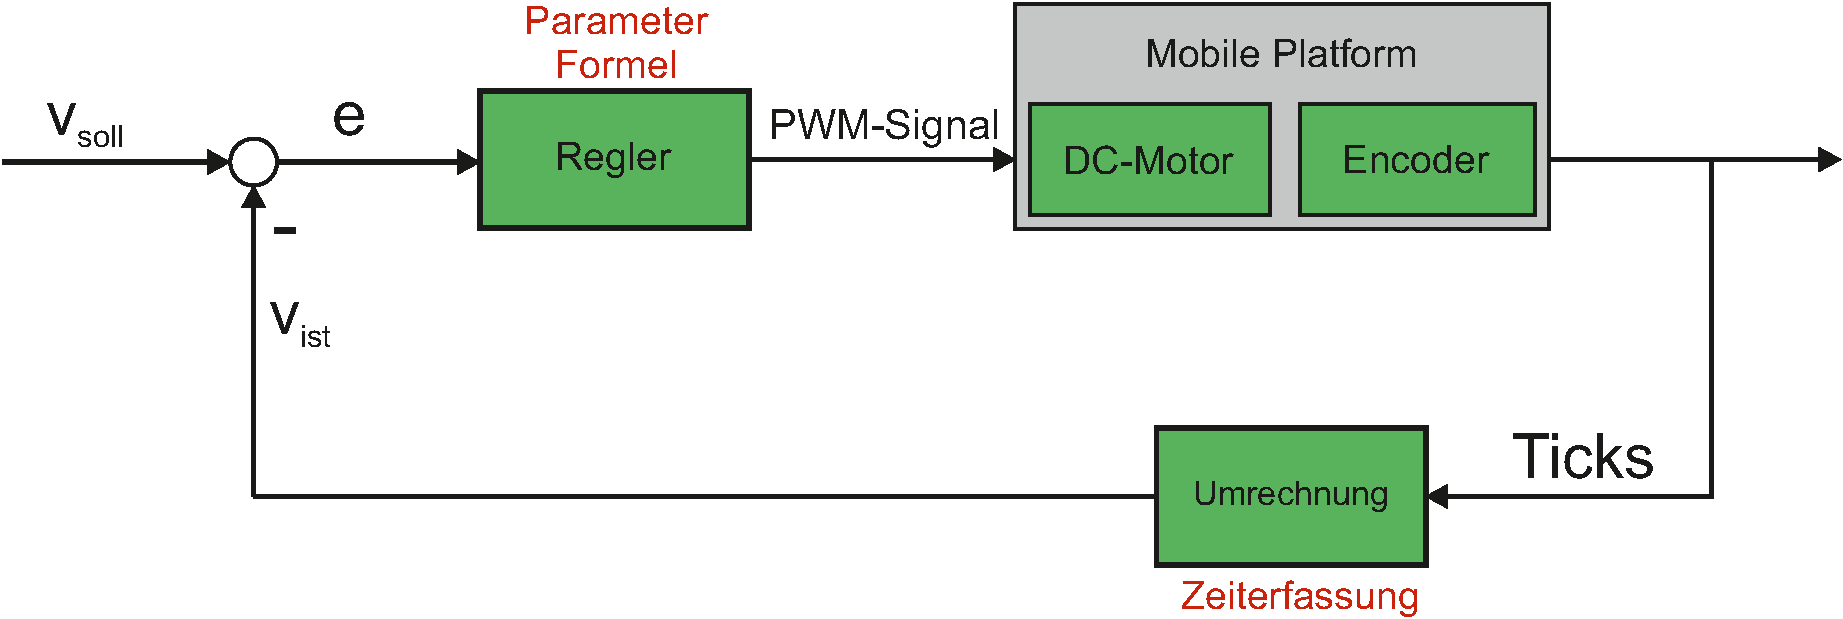
\includegraphics[scale=.5]{figs/PID_controller}
	\caption{Blockschaltbild eines PID-Reglers}
	\label{fig:PID_controller}
\end{figure}

Die Eingangsgröße des Reglers ergibt sich aus der Differenz und somit dem Fehler $e$ aus Ist-Geschwindigkeit $v_{ist}$ und Soll-Geschwindigkeit$v_{soll}$. Diese Differenz wird nach Formel \ref{eq:pidController} durch einen proportionalen , integralen und differentiellen Anteil so verstärkt, dass sich die Regelabweichung verkleinert und im optimalen Fall verschwindet. Der proportionale Anteil verstärkt dabei den Fehler mit einem konstanten Faktor $K_{P}$. Da der es sich um einen zeit diskreten Regler handelt, bildet sich der integrale Anteil nicht durch eine Integration der Regelabweichung über die Zeit, sondern. durch die Multiplikation der Summe aller Fehler mit der Konstanten $K_{I}$. Analog dazu wird der differenzielle Anteil nicht nach der Zeit abgeleitet sondern ergibt sich aus dem Produkt der Differenz des Fehlers mit dem Fehler des vergangenen Abtastschrittes und dem Faktor $K_{D}$. 

\begin{center}
	\begin{equation}
	y[n] =  K_{P}\cdot e[n] + K_{I} \cdot \sum\limits_{m=0}^n e[m] \cdot \Delta T+ K_{D} \cdot \frac{e[n] - e[n-1]}{\Delta T}
	\label{eq:pidController}
	\end{equation}
\end{center} 

Die Verstärkungen der Regler werden über $Live-Tuning$, das heißt im laufenden Betrieb des Roboters ermittelt. Eine Auslegung der Parameter über ein lineares Systemmodell zweiter Ordnung ist nur schwer möglich, da das Übertragungsverhalten von Geschwindigkeit und PWM-Signal nichtlinear ist. Dieses Verhalten ist in der Kennlinie von Abbildung \ref{fig:nl_kennlinie_R} zu entnehmen.
Des Weiteren wurden für beide Motoren verschiedene Parameter ermittelt, da sie bei gleichem Eingangssignal unterschiedliche Drehzahlen aufweisen. 

\begin{figure}[!htb]
	\centering
	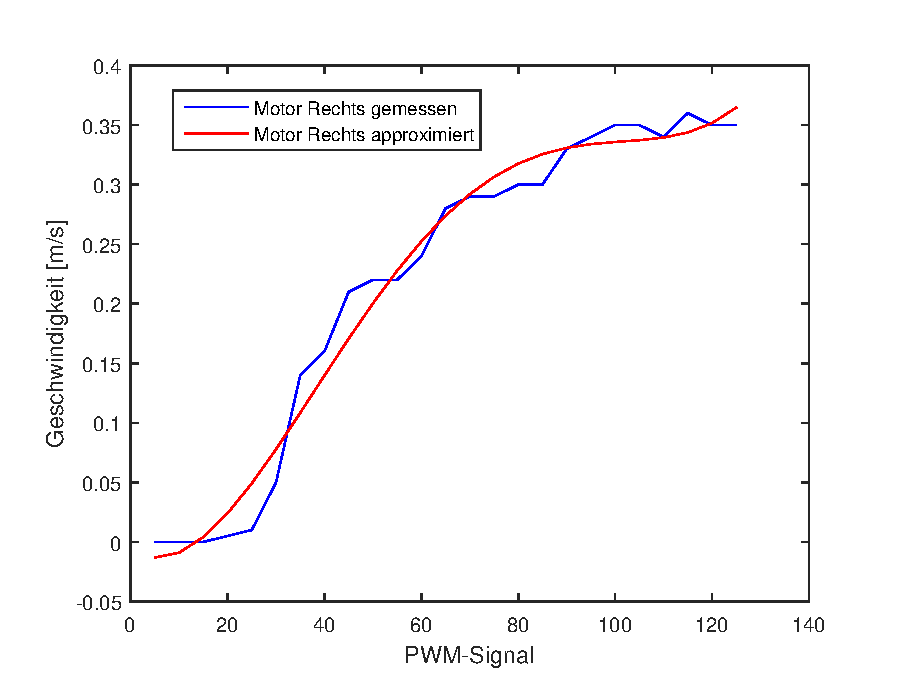
\includegraphics[scale=.7]{figs/Motor_Rechts_Kennlinie.eps}
	\caption{Nichtlineare Kennlinie der Drehzahl des rechten Motors}
	\label{fig:nl_kennlinie_R}
\end{figure}

\newpage
Zur Realisierung der Kreisfahrt im Uhrzeigersinn wurde die Klasse \textit{Mobileplatform} um eine Methode erweitert, die eine Funktion zur Berechnung der einzelnen Radgeschwindigkeiten bereitstellt. Die Basisgeschwindigkeit wird dabei zwischen beiden Rädern angenommen (Abbildung \ref{fig:kreisfahrt}), deren Abstand ($b=11cm$) beträgt. Da die Distanz von Mittelpunkt zu Stifthalter ($s = 12 cm$), welcher am hinteren Ende des Roboters befestigt wurde, nicht vernachlässigbar ist, fließt dessen Position in die Berechnung der Geschwindigkeiten mit ein. Aus Abbildung \ref{fig:kreisfahrt}, die eine Rotation des Roboters um einen Punkt P darstellt, folgen die Gleichungen \ref{eq:kreisfahrt1}, \ref{eq:kreisfahrt2} und \ref{eq:kreisfahrt3} zur Berechnung der Soll-Geschwindigkeiten.

\begin{center}
	\begin{equation}
		r_{soll} = \sqrt{r^2-s^2}
	\label{eq:kreisfahrt1}
	\end{equation}
\end{center} 

\begin{center}
	\begin{equation}
	v_{Links} = v \cdot \frac{r + \frac{b}{2}}{r}
	\label{eq:kreisfahrt2}
	\end{equation}
\end{center} 

\begin{center}
	\begin{equation}
	v_{Rechts} = v \cdot \frac{r - \frac{b}{2}}{r}
	\label{eq:kreisfahrt3}
	\end{equation}
\end{center}


\begin{figure}[!htb]
	\centering
	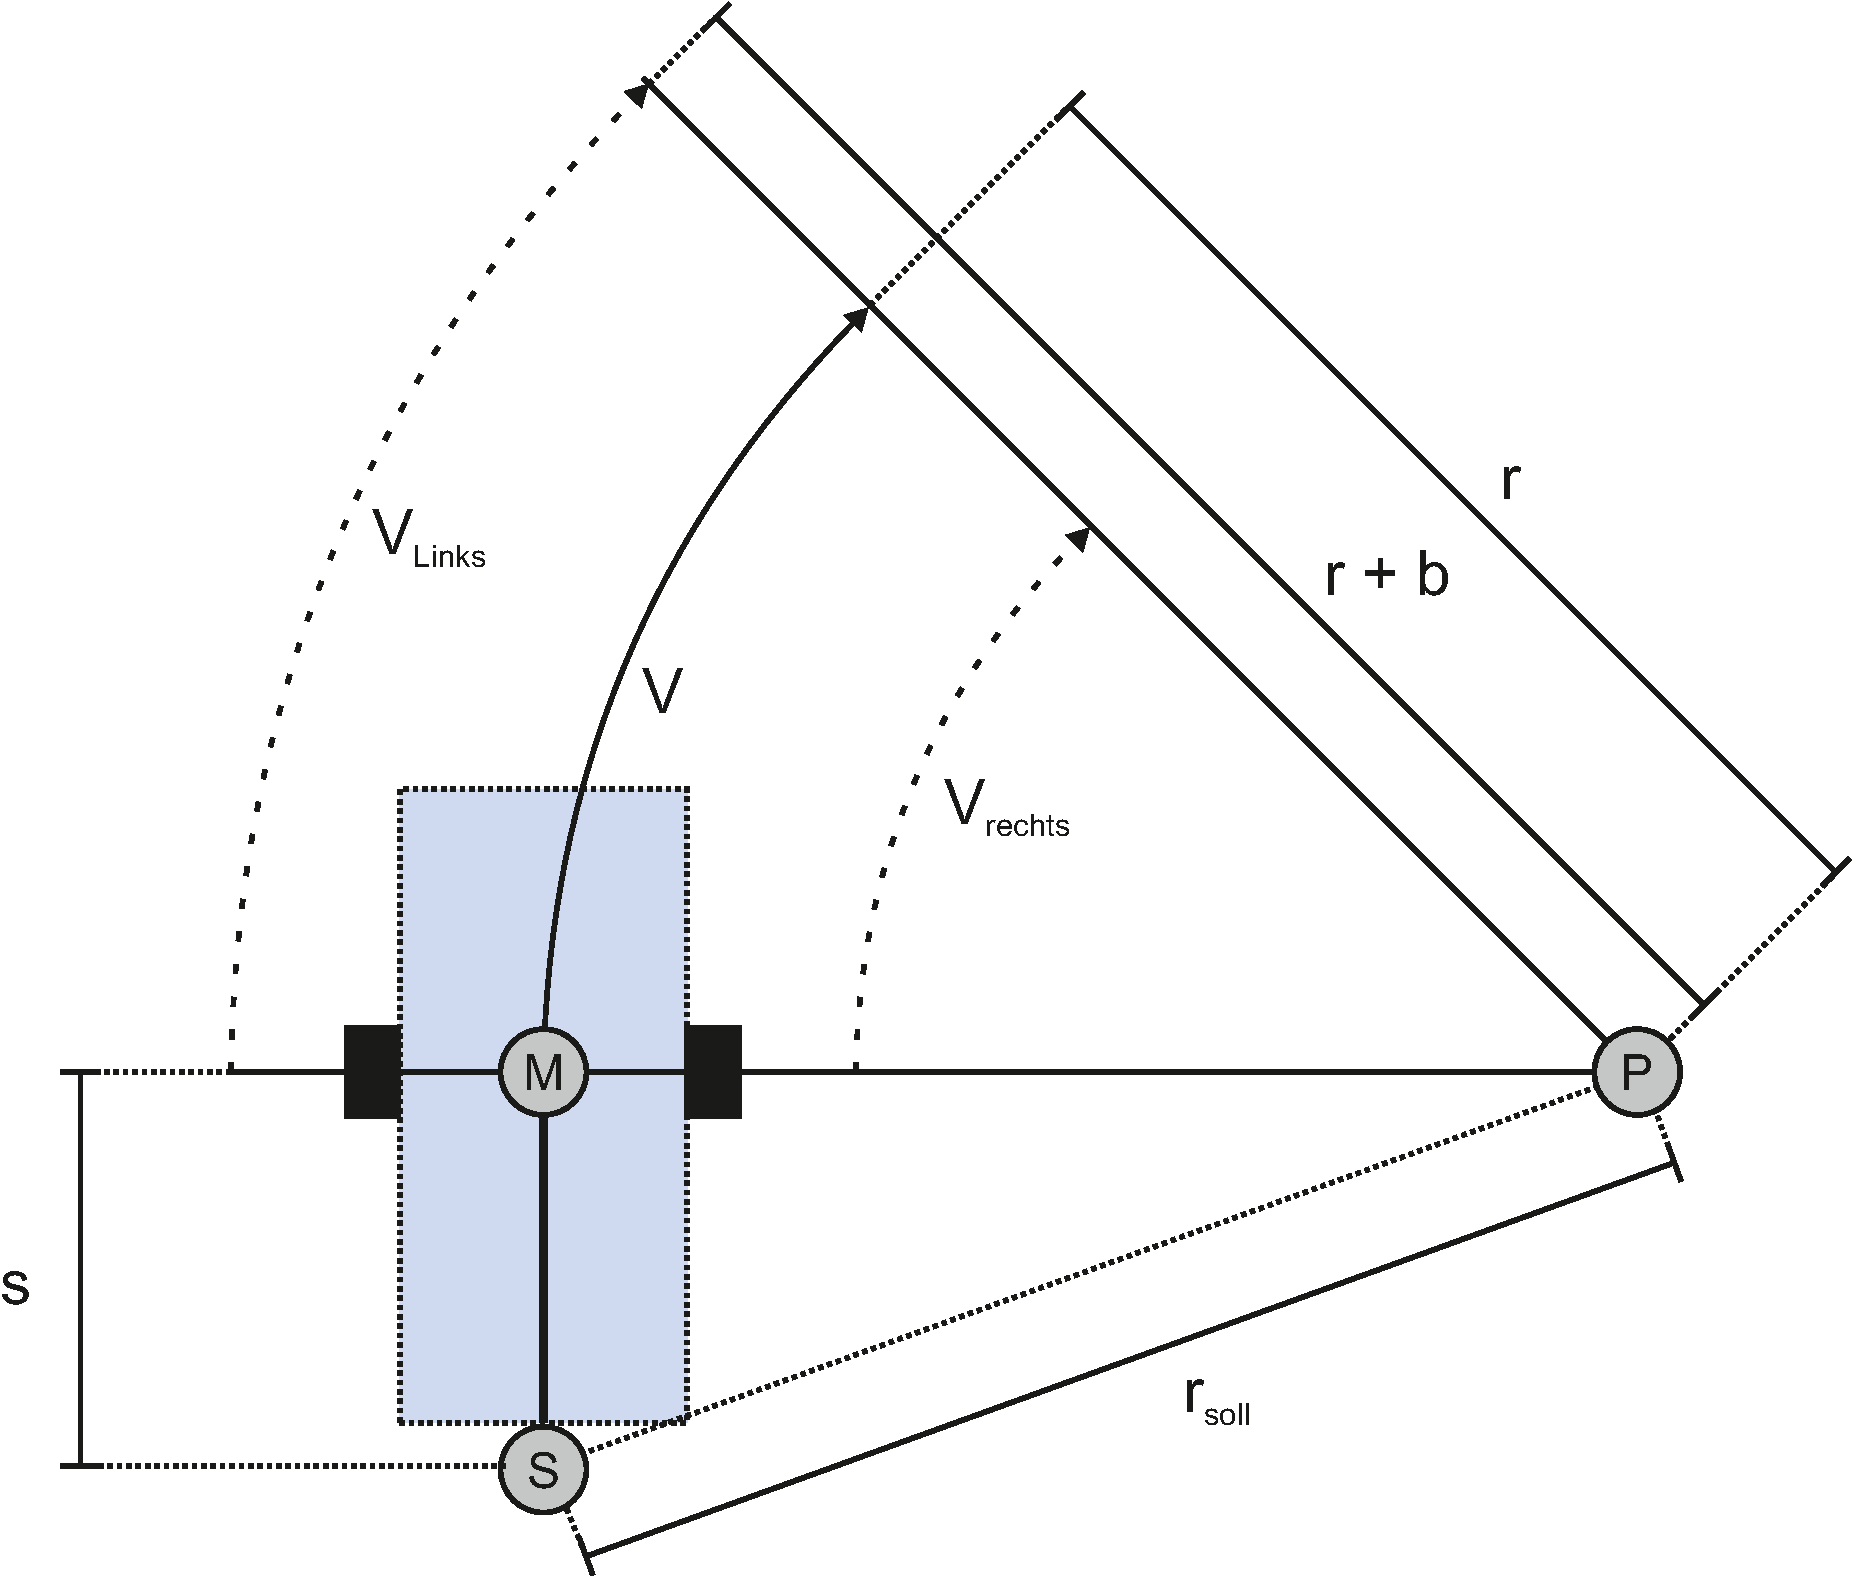
\includegraphics[scale=.4]{figs/Kreisfahrt}
	\caption{Nichtlineare Kennlinie der Drehzahl des rechten Motors}
	\label{fig:kreisfahrt}
\end{figure}


\newpage
Bei der Abnahme des Meilensteins wurden Radien von 23 und 30 cm abgefahren. Dies lief bei $r_{soll} = 23 cm$ problemlos. Nur beim Radius von 30 cm gab es kleine Überschreitungen der Toleranzgrenze von $\pm$ 2cm. Da die Signale der Encoder ausreichend hochauflösend sind, ist dieser Fehler hauptsächlich auf die Einschwingvorgänge des Reglers und Messunsicherheiten der Geometrien zurückzuführen. 

In den weiteren Aufgabenteilen wird die Geschwindigkeitsregelung beibehalten, da sie die Laufruhe des Roboters unterstützt und auch dabei hilft Hindernisse zu überwinden.




	
\subsection{Kollisionsfreie Korridorfahrt}

Herausforderung des 3. Meilensteins war eine kollinsionsfreie Fahrt durch ein Labyrinth mit einem konstanten Wandabstand von 35 cm. Die Rechts- und Linksabbiegungen der Strecke verlaufen dabei alle mit einem Winkel von 90 Grad. Zur Messung des absoluten Abstands von Roboter zu Wand wurden zwei Ultraschallsensoren (siehe Kapitel 2.2) angeschlossen und aus einer Klasse \textit{Ultrasonic} angesprochen. Die Sensoren werden nacheinander ausgelesen um Interferenzen und somit Fehler bei der Distanzmessung zu vermeiden. Des weiteren wurden die Ultraschallsensoren nicht direkt seitlich an der Plattform angebracht, sondern mit einem leichten Winkelversatz von 30 Grad nach vorne montiert. Abbildung \ref{fig:kurve} zeigt, dass dies ein Vorausschauen des Roboters und somit die rechtzeitige Erkennung von Abbiegungen bewirkt. Zudem verringert diese Art der Anbringung Messunsicherheiten des Ultraschallsensors, die sich auf schrägen Oberflächen einstellen.

\begin{figure}[!htb]
	\centering
	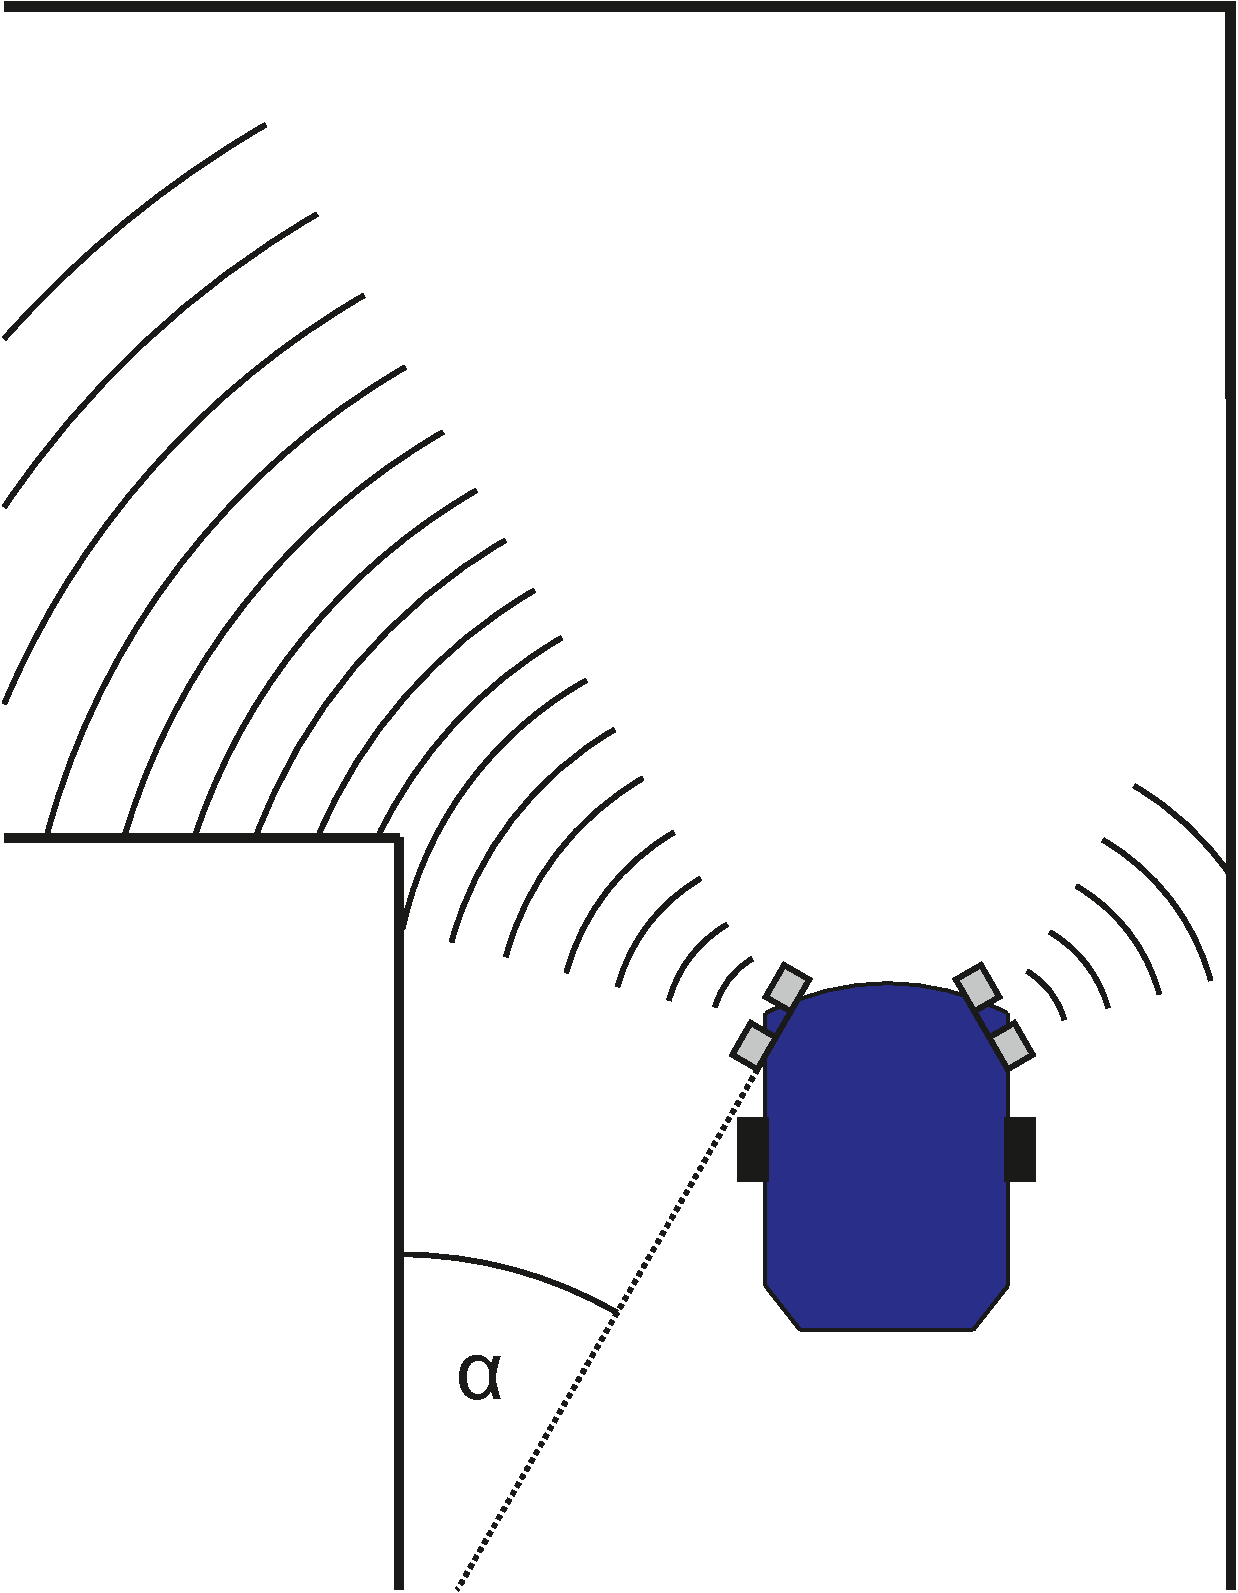
\includegraphics[scale=.3]{figs/kurve}
	\caption{Anbringung der Ultraschallsensoren im Hinblick auf Kurvenverhalten}
	\label{fig:kurve}
\end{figure}

Das UML-Diagramm in Abbildung ... veranschaulicht, den Zusammenhang der Klasse \textit{Mobileplatform} und \textit{Ultrasonic}. Es ist ersichtlich, dass \textit{Mobileplatform} vollständigen zugriff auf Funktionalitäten der Ultraschallsensoren erhält. Somit eignet sich diese Klasse gut für die Implementierung des Algorithmus zur Korridorfahrt, der die Erkennung von Hindernissen gewährleisten soll. Zur Regelung des Roboters während der Fahrt wurden im Rahmen dieser Arbeit drei verschiedene Ansätze mir unterschiedlicher Anordnung der Ultraschallsensoren erprobt. Diese verschiedenen Strategien werden im Folgenden erläutert und mit Abbildung \ref{fig:ansatz} unterstützt.

\begin{figure}[!htb]
	\centering
		\subfigure[Berücksichtung Winkelversatz]
		{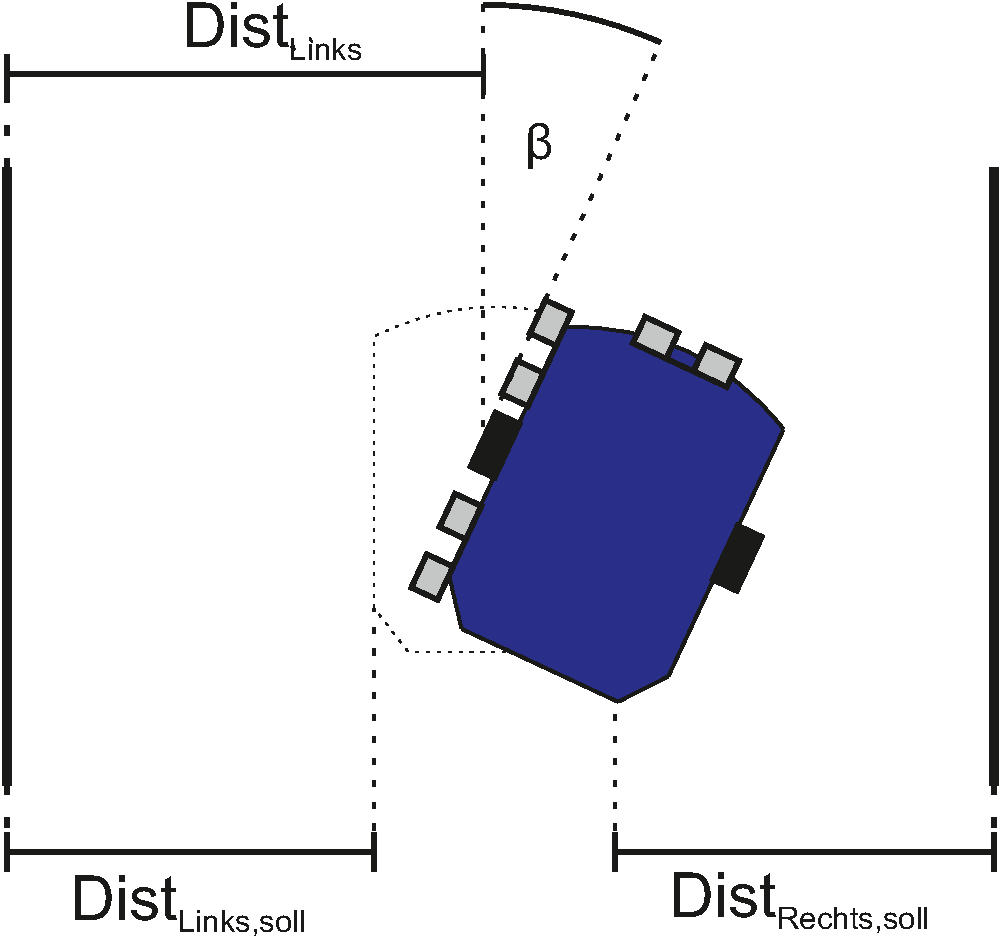
\includegraphics[scale=.35]{figs/ansatz2}}
	\hspace{5mm}
	\subfigure[Distanzmessung beider Seiten]
	{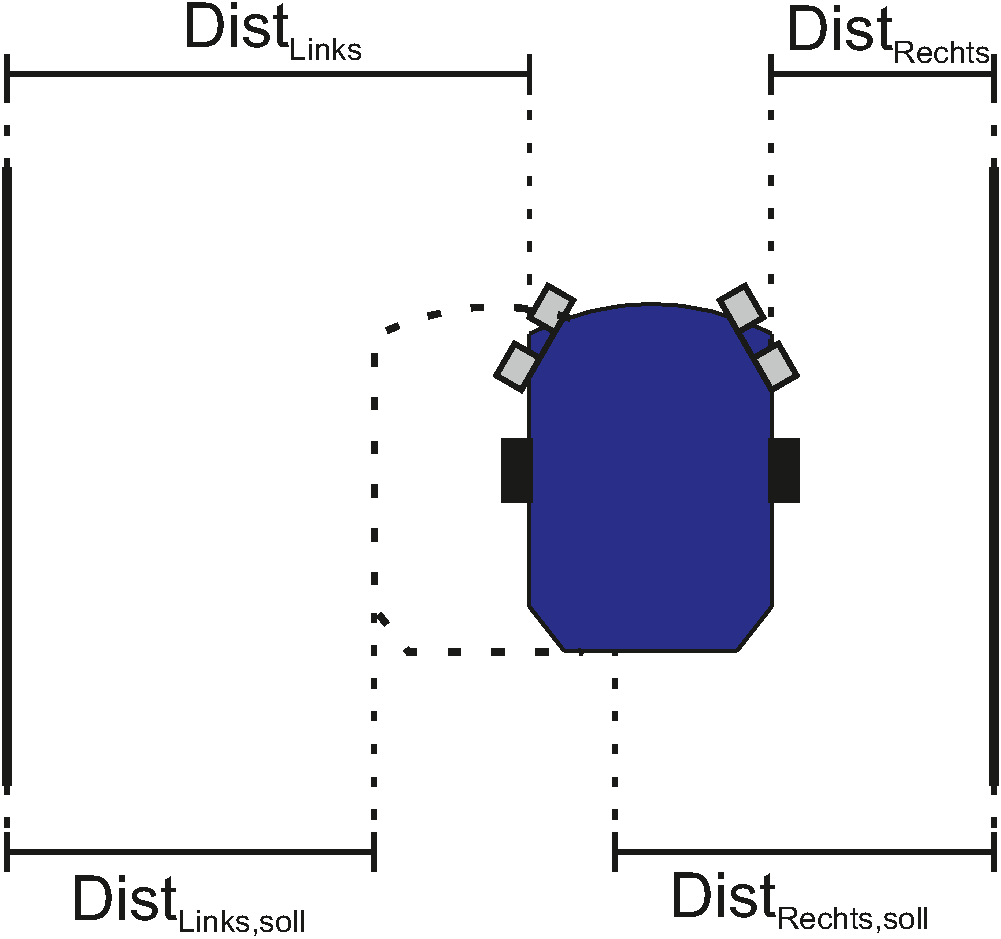
\includegraphics[scale=.35]{figs/ansatz}}
	\caption{Position des Roboters im Korridor}
	\label{fig:ansatz}
\end{figure}

In Abbildung \ref{fig:ansatz}(a) sind zwei Sensoren seitlich am Roboter montiert und einer in Fahrtrichtung. Der Ansatz des Algorithmus beruht auf einer Orientierung an der Linken Wand des Korridors. Dabei werden wird sowohl der Winkelversatz, als auch der Abstand zur Wand in der Fahrt des Roboters berücksichtigt und korrigiert. Der vordere Sensor detektiert, ob sich ein Hindernis in Fahrtrichtung befindet und ein Abbiegevorgang ausgeführt werden muss. \\
Der zweite und dritte erprobte Ansatz wird mit der zuvor beschriebenen winkelversetzten Sensorkonfiguration ausgeführt. Beide Ansätze beruhen darauf eine Soll-Distanz zu beiden Wänden einzuhalten und den Roboter somit mittig im Korridor zu halten (Abbildung \ref{fig:ansatz}). \\
Dies wurde im Rahmen des zweiten Ansatzes dadurch realisiert, das Verhältnis aus $Dist_{Links}$ und $Dist_{Rechts}$ mit der Initialgeschwindigkeit beider Motoren zu multiplizieren. Somit ergeben sich nach Gleichung \ref{eq:verhaeltnis1} und \ref{eq:verhaeltnis2} für beide Räder neue Soll-Geschwindigkeiten. Diese Geschwindigkeiten sind dabei auf einen Bereich zwischen $0,05$ und $0.4$ Meter pro Sekunde begrenzt.

\begin{center}
	\begin{equation}
	v_{Rechts} = v \cdot \frac{Dist_{Links}}{Dist_{Rechts}}
	\label{eq:verhaeltnis1}
	\end{equation}
\end{center}

\begin{center}
	\begin{equation}
	v_{Links} = v \cdot \frac{Dist_{Rechts}}{Dist_{Links}}
	\label{eq:verhaeltnis2}
	\end{equation}
\end{center} 

Da sich bei Abbiegungen ein entsprechend großes Verhältnis einstellt, ist dieser Ansatz auch für Abbiegevorgänge geeignet. \\
Als dritte Option, wurde eine Abstandsregelung mittels zweier P-Regler implementiert. Diese setzte sich im aufgrund ihrer Robustheit und sich einstellenden Fahrtruhe gegen die zuvor genannten Verfahren durch. Da die Ultraschallsensoren, aufgrund ihrer Positionierung nicht den direkten Abstand zur Wand messen, wurde zur Bestimmung der Soll-Größen eine Referenzmessung durchgeführt, bei der der Roboter mittig im Korridor platziert wurde. Somit ergab sich bei mittiger Fahrt eine minimale Regelabweichung $e$. Ein Blockdiagramm des verwendeten P-Reglers ist in Abbildung ... zu sehen.\\
Die Ermittlung der proportionalen Regelverstärkung erfolgte empirisch. Dabei musste ein Kompromiss aus steiler Kurveneinlenkung und ruhiger Geradeausfahrt gefunden werden. Abbildung ... zeigt, dass sich bei geringen Verstärkungen der Regeldifferenz zwar ein ruhiges Fahrverhalten auf gerader Strecke ergibt, das Einlenken in Kurven jedoch durch zu träge ist und zu Kollisionen führen kann. Analog dazu ergibt sich bei großer Fehlerverstärkung eine ungleichmäßige, zur Seite schwingende Geradeausfahrt, die bis zum Kontakt mit den Seitenwänden führen dann. In Kurven agiert der Roboter hingegen hoch dynamisch (Abbildung ...).

\begin{figure}[!htb]
	\centering
	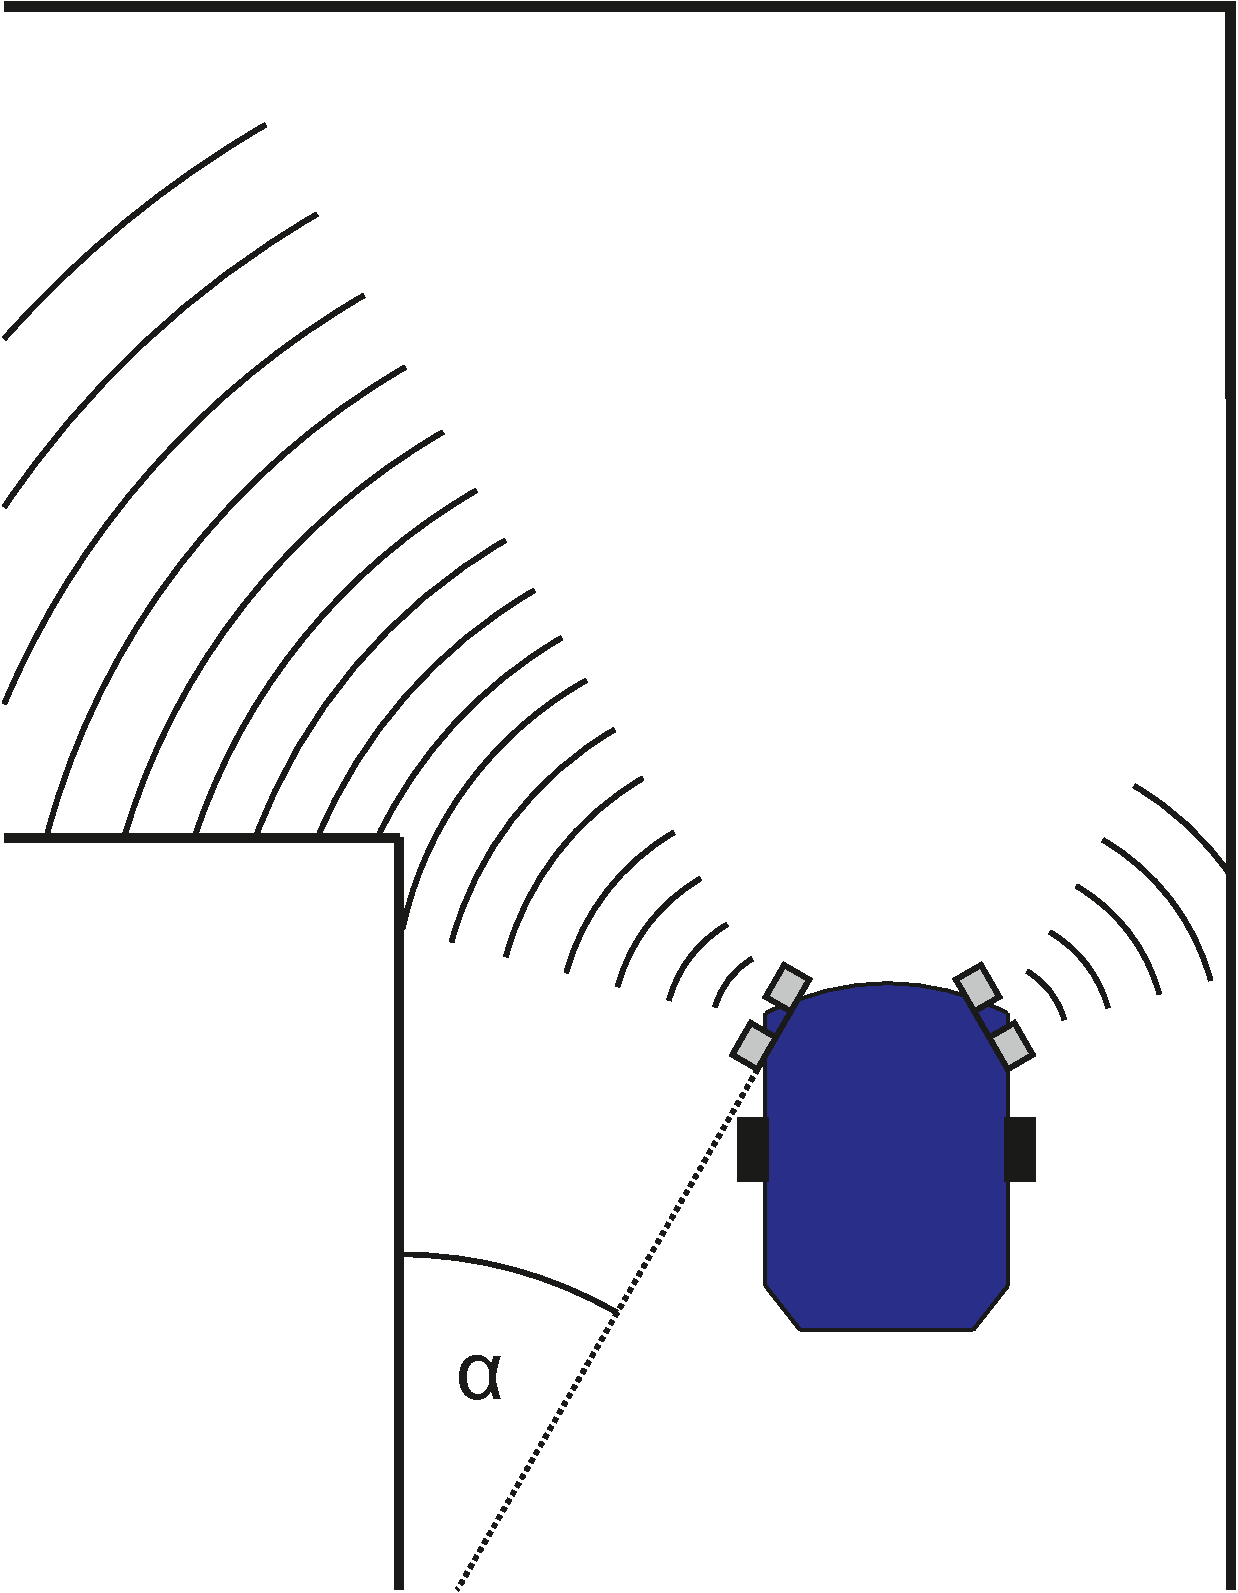
\includegraphics[scale=.3]{figs/kurve}
	\caption{Anbringung der Ultraschallsensoren im Hinblick auf Kurvenverhalten}
	\label{fig:kurve}
\end{figure}

\newpage

\subsection{Farbfeld-Suche}
	
Beim letzten Meilensteins, der auch als "Roboter-Challenge" bezeichnet wird, handelt es sich um eine Erweiterung der kollisionsfreien Korridorfahrt. Die abzufahrende Strecke wird vergrößert und um weitere Abbiegungen erweitert, welche nicht mehr nur um 90 Grad, sondern auch in einem beliebigen Winkel abknicken können. Zudem werden im Labyrinth Hindernisse in Form einer Wippe und einer Bodenwelle verteilt und Farbfelder in den Farben Rot, Grün und Blau ausgelegt. Die Hindernisse sind ohne weitere Veränderung des Algorithmus zu bewältigen, was auf den Geschwindigkeitsregler zurückzuführen ist, der einer Verringerung der Geschwindigkeit auf einer Steigung entgegenwirkt. Die Farbfelder der werden über einen RGB-Farbsensor des Typs "FLORA Color Sensor" detektiert. Über eine Klasse \textit{Colorsensor}, die in der \textit{Mobileplatform}  implementiert ist, können die einzelnen RGB-Farben über 16-Bit-Integer ausgelesen werden.
Der Parkour ist dann erfolgreich abgeschlossen, wenn der Roboter ohne Kollisionen über die Hindernisse fährt und schließlich auf dem roten Farbfeld stehen bleibt. 

Da für die Parkourfahrt nur das rote Farbfeld von Bedeutung ist, wird die Farbe Rot nach im Verhältnis zu Grün und Blau identifiziert. Die dabei benutzten Schwellenwerte wurden dabei empirisch ermittelt. 
	
	%-----------------------------
	% Diskussion
	%-----------------------------
	\section{Diskussion}
	\textit{0.5 bis 1 Seite}
	\textit{Probleme mit Hardware/Software, Herausforderungen die euch begegnet sind, Probleme im Team, Warum hat euer Roboter in der Challenge wie abgeschnitten? Gibt es offene Fragen? Wenn ihr jetzt noch weiter daran arbeiten könntet, was würdet ihr als nächstes machen?}
	
	%-----------------------------
	% Zusammenfassung
	%-----------------------------
	\section{Zusammenfassung}
	\textit{0.5 Seite}
	
	
	\clearpage  
	\begin{appendix}
	\section{Programmcode}
	\end{appendix}
    \clearpage  
    %% --- Literaturverzeichnis
    \begin{thebibliography}{50}
   		\bibitem{Dem13} Klaus Dembowski: \textit{Raspberry Pi - Das Handbuch}. Springer Vieweg, ISBN 978-3-658-03166-4, 2013.
	\end{thebibliography}

\end{spacing}
\end{document}                             

